\chapter{Bezier Curves} 
Invented by Pierre Bezier (Renault) and Pierre De Casteljau (Citreon). 
No interpolation points, rather we have "control points". 

\section{Bernstein Polynomials}
\label{sec:Bernstein Polynomials}
\begin{defn}[Bernstein Polynomials]
    $ \\ $
    Let $ n \in \mathbb{N}  $ and $ i \in \set{ 0, \dots, n  }  $. Then the Bernstein
    polynomials are given by 
    \[
        B^n_i(t) = \begin{pmatrix*}
             n \\
             i 
        \end{pmatrix*}
        t^i \left( 1 - t\right) _{  }^{ n-i } 
    \] where 
    \[
    \begin{pmatrix*}
         n \\
         i 
    \end{pmatrix*}
    = \frac{ n! }{ i! \left( n - i\right) ! } 
    \]
    \label{def:bernsteinPoly}
\end{defn}
\subsection{Properties}
\label{subsec:Properties}
\begin{enumerate}[label={(\alph*)}]
    \item Positivity : 
        \[
            \forall i \ B^n_i(t) \geq 0
        \]
    \item Partition of unity : 
        \[
            \sum_{i=0}^{n} B^n_i (t) = 1
        \]
    \item Linear precision : 
        \[
            \sum_{i=0}^{n} \frac{ i }{ n  } B^n_i(t) = t
        \]
    \item Recursion Formula : for $ 0 \leq i \leq n $
        \[
            B^n_i(t) = \left( 1-t\right) B _{ i }^{ n-1 } (t) + B _{ i-1 }^{ n-1 } (t) 
        \]
        with the convention that $ B _{ j }^{ n  } = 0  $ if $ j \notin [0,n] $
    \item Symmetry : 
        \[
        B _{ i }^{ n  } = B _{ n- i  }^{ n  } \left( 1-t \right) 
        \]
    \item Derivative : 
        \[
            B _{ i }^{ n  } '(t) = n \left( B _{ i-1  }^{ n-1 } (t) - B _{ i }^{ n-1 } (t) \right) 
        \]
    \item Extremum : 
        $ \\ B _{ i }^{ n   } $ has an extremum at $ t = \frac{ i }{ n  }  $
    \item Basis : 
        \[
            \set{ B _{ i }^{ n  } , 0\leq i \leq n  } \text{ is a basis of }
            \mathbb{R}_n[x]
        \]
\end{enumerate}

\subsubsection{a) }
ok 

\subsubsection{b)}
\[
    \sum_{i=0}^{n} B _{ i }^{ n } = \sum_{i=0}^{n} 
    \begin{pmatrix*}
        n \\
        i 
    \end{pmatrix*}
    t^i\left( 1 - t\right) ^{n-i} 
\]
Using the binomial theorem, which states that 
\[
    \left( a+b\right) ^n
\sum_{i=0}^{n} \begin{pmatrix*}
    n \\
    i 
\end{pmatrix*}
a^ib^{n-i} 
\] 
Therefore, we have 
\[
\left( t + \left( 1 - t\right) \right) ^n = 1
\]


\subsubsection{c)}
?


\subsubsection{d)}
We have, from definition of binomial that 
\[
\begin{pmatrix*}
     n \\
     i-1
\end{pmatrix*}
+ 
\begin{pmatrix*}
     n \\
     i
\end{pmatrix*}
=
\begin{pmatrix*}
    n+1  \\
    i  
\end{pmatrix*}
\]

Expanding the original equation and simplifying the coefficents. 

\[
\begin{pmatrix*}
    n   \\
    i  
\end{pmatrix*}
t^i\left( 1-t\right) _{  }^{ n-i } = \begin{pmatrix*}
    n-1  \\
    i  
\end{pmatrix*}
t^i\left( 1-t\right) _{  }^{ n-i } + \begin{pmatrix*}
    n-1  \\
    i-1  
\end{pmatrix*}
t^{i}\left( 1-t\right) ^{n-i} 
\]
We now have 
\begin{align*}
    &\left( \begin{pmatrix*}
        n-1  \\
        i-1  
    \end{pmatrix*}
    + 
    \begin{pmatrix*}
        n-1  \\
        i  
    \end{pmatrix*}
\right) t^i\left( 1-t^{n-i} \right) \\
 &= \begin{pmatrix*}
     n   \\
     i  
 \end{pmatrix*}
 t^i\left( 1-t\right) ^{n-i}   \\ 
 &= B _{ i }^{ n  } (t) \\ 
\end{align*}

\subsubsection{e) }
We have from properties of binomials that 
\[
\begin{pmatrix*}
    n   \\
    k  
\end{pmatrix*}
= \begin{pmatrix*}
    n   \\
    n-k  
\end{pmatrix*}

\]
Then 
\begin{align*}
    B _{ n-i }^{ n } \left( 1 - t\right) &= 
\begin{pmatrix*}
     n \\
     n-i  
\end{pmatrix*}
\left( 1-t\right) ^{n-i} \left( 1-(t-1)\right) ^{ n - (n-i)} \\
                                         &= \begin{pmatrix*}
                                             n   \\
                                             i  
                                         \end{pmatrix*}
                                         t^i \left( 1-t\right) _{  }^{ n-i } 
\end{align*}

\subsubsection{f)}
\[
    n \left( B _{ i-1 }^{ n-1 } (t) - B _{ i }^{ n-1 } (t)\right) 
\]
\[
= n \begin{pmatrix*}
     n-1 \\
     i-1 
\end{pmatrix*}
t^{i-1} \left( 1-t\right) ^{n-i} - n \begin{pmatrix*}
    n-1 \\
     i 
\end{pmatrix*}
t^i \left( 1-t\right) ^{n-1-i} 
\]
\[
= i \begin{pmatrix*}
     n \\
     i 
\end{pmatrix*}
t^{i-1} \left( 1-t\right) ^{n-i} -  \begin{pmatrix*}
    n \\
     i 
\end{pmatrix*}\left( n-i \right) 
t^i \left( 1-t\right) ^{n-1-i} 
\]
\[
=  \begin{pmatrix*}
     n \\
     i 
\end{pmatrix*}
t^{i-1} \left( 1-t\right) ^{n-1-i} 
\left( i\left( 1-t\right) - \left( n-i\right) t\right)          
\]
\[
= \begin{pmatrix*}
    n  \\
    i 
\end{pmatrix*}
t ^{i-1} \left( 1-t\right) ^{n-1-i} \left( i-tn \right) 
\]
On the other hand 
\[
    B' _{ i }^{ n  } (t) = \begin{pmatrix*}
         n \\
         i 
    \end{pmatrix*}
    \left( it^{i-1} \left( 1-t \right) ^{n-i} - t^i \left( 1-t\right) ^{n-i-1} \left(
    n-i\right) \right) 
\]
\[
= \begin{pmatrix*}
     n \\
     i 
\end{pmatrix*}
t^{i-1} \left( 1-t\right) ^{n-1-i} \left( i\left( 1-t\right) -t\left( n-i\right) \right) 
\]

\section{Bezier Curves}
\label{sec:Bezier Curves}
\subsection{Refresher on Convex Hull and Barycenter}
\label{subsec:Refresher on Convex Hull}
\begin{prop}[]
    Let $ p_1, \cdots, P_n \in \mathbb{R}^d $ and $ \lambda_1, \cdots , \lambda_n \in
    \mathbb{R} $ and $ \sum_{i=1}^{n} \lambda_i \neq 0 $
    \[
    \exists ! \in \mathbb{R}^d , \sum_{i=0}^{n} \lambda_i \boldsymbol{GP} _i =
    \boldsymbol{0} 
    \]
    G is given by 
    \[
    \boldsymbol{OG} = \frac{ \sum_{i=1}^{n} \lambda_i \boldsymbol{OP} _i }{ \sum_{i=1}^{n}
    \lambda_i } 
    \]
    G is called the barycenter of $ P_i $ with weight $ \lambda_i $
    \label{prop:}
\end{prop}
\begin{proof}
    Let $ o \in \mathbb{R}^d  $ be any point 
    \begin{align*}
        \boldsymbol{o}  &= \sum_{i=1}^{n} \lambda_i \boldsymbol{GP} _i = \sum_{i=1}^{n}
        \lambda_i\left( \boldsymbol{GO} + \boldsymbol{OP_i} \right)   \\ 
         &= \left( \sum_{i=1}^{n} \lambda_i\right) \boldsymbol{GO} +
         \sum_{i=1}^{n}\lambda_i \boldsymbol{OP_i}   \\ 
    \end{align*}
    
\end{proof}


\begin{defn}[Convec Set]
    $ K \subset \mathbb{R}^d $ is convex if 
    \[
        \forall x,y \in K, \quad [x,y] \subset K
    \]
    \label{def:Convec Set}
\end{defn}

\begin{defn}[Convex Hull]
    Denoted 
    \[
        \text{Conv}\left( K\right) = \cap_{K \subset K'} K' 
    \]
    The smallest convex set that contains the set
    \label{def:Convex Hull}
\end{defn}

\begin{prop}[]
    $ A = \set{ p_1, \cdots, p_n }  $ then 
    \[
    \text{Conv } \left( A\right) = \set{ \sum_{i=1}^{n} \lambda_ip_i, \sum_{i=1}^{n}
    \lambda_i = 1, \ \lambda_i \geq 0 } 
    \]
    is the set of barycenter with positive weights
    \label{prop:}
\end{prop}

\begin{proof}
    Let 
    \[
    F = \set{ \sum_{}^{} \lambda_ip_i, \sum_{}^{} \lambda_i = 1, \lambda_i \geq 0 } 
    \]
    Conv $ (A) \subset F $, F convex. 
    \begin{align*}
        m \in F &\implies m = \sum_{}^{} \lambda_ip_i  \\ 
        n \in F &\implies m = \sum_{}^{} \lambda_i'p_i  \\ 
    \end{align*}
    \[
        q \in [m,n] \implies q = tm + (1-t)n \ t\in [0,1]
    \]

    So 
    \[
        q = \sum_{i=1}^{n} \underbrace{\left( t\lambda_i + \left( 1-t\right)
            \lambda_i'\right)  }_{\lambda_i'' \geq 0}p_i \in F
    \] 
    Then $ [m,n] \subset F $. $ F\subset A $ and $ \lambda''_i = 1 $

    $ \\ $
    $ F \subset \text{Conv}(A) $
    By recursion $ P(n) : $ every barycenter of n points $ q_1, \cdots, q_n  $ belong to
    Conv($q_1, \cdots, q_n)  $. $ \\ $
    n = 1 : 
    $ \\ $
    Let $ n \geq 1  $ $ Sq P(n) $ 
    $ \\ $
    Let $ p_1, \cdots, p_{n+1}  $ points of $ \mathbb{R}^d $ and $ \lambda_1, \cdots,
    \lambda_{n+1} \in \mathbb{R}^d $ with sum = 1. and 
    \[
        m = \sum_{i=1}^{n+1} \lambda_ip_i = \sum_{i-1}^{n} \lambda_ip_i +
        \lambda_{n+1}p_{n+1} + 1
    \]
    Let $ g $ denote the barycenter of $ p_1, \cdots, p_n  $ with associated $ \lamda_i  $
    then 
    \[
    \sum_{i=1}^{n} \lambda_ip_i = \left( \sum_{i=1}^{n} \lamda_i\right) g
    \]
    \[
        = \left( 1-\lambda_{n+1} \right) g
    \]
    then 
    \[
        m = \left( 1-\lambda_{n+1}\right) g + \lambda_{n+1}p_{n+1} \in [g, p_{n+1} ] 
    \]
    by assumption $ g\in \text{Conv}\left( A\right)  \implies m \in \text{Conv}\left(
    A\right)   $.

\end{proof}

\begin{exmp}[]
    \[
        [p_1, p_2] = \set{ tp_1 + \left( 1-t\right) p_2, t\in [0,1] } 
    \]
\end{exmp}



\begin{defn}[]
    We see $ \mathbb{R}^d $ is both affine and vector space. 
    \begin{itemize}
      \item $ p\in \mathbb{R}^d $ is a point 
      \item $ p-q = \boldsymbol{pq}  $ is a vector  
  \end{itemize}
    \label{def:}
\end{defn}

In particular $ \sum_{i=1}^{n} \lambda_ip_i = 0 $ gives a vector, barycenter otherwise(a
point). 


\subsection{Definition of Bezier Curves}
\label{subsec:Definition of Bezier Curves}
Let $ p_0, \cdots, p_n $ points of $ \mathbb{R}^d,\ n > 0 $. The Bezier curve associated
to $ p_0, \cdots, p_n $ is the parametrized curve
\begin{align*}
    P:[0,1] &\rightarrow \mathbb{R}^d  \\ 
    t &\rightarrow \sum_{i=0}^{n} P_iB_i^n(t)
\end{align*}
We call $ [P_o, \cdots, P_n] $ the Bezier control polygon. 

\begin{exmp}[n=1]
    \[
        P(t) = p_0B _{0 }^{ 1 }(t) + B _{ 1 }^{ 1 } (t) 
    \]
    \[
    = p_0t + p_1\left( 1-t\right) 
    \]
    P is a parametrization of $ [p_0, p_1] $
\end{exmp}


\subsection{Properties}
\label{subsec:Properties}
\begin{enumerate}[label={(\alph*)}]
    \item boundary : 
        \[
            P(0) = P_0 \qquad \text{ and } P(1) = P_n
        \]
        \begin{proof}
            \[
                P(0) = \sum_{i=0}^{n} B _{ i }^{ n  } (0)P_i = P_0 
            \]
        \end{proof}
    \item Convex Hull : 
        \[
            P\left( [0,1]\right) \subset \text{Conv}\left( \text{control polygon} \right)  
        \]
        \begin{proof}
            $ \forall t \in [0,1] $ $ P(t) = \sum_{i=0}^{n} B _{ i }^{ n }(t) P_i   $
            where $ B _{ i }^{ n  }  $ is $ \lambda_i  $ which is positive and the sum of
            which is equal to one. Therefore, P belongs to the convex hull. 
        \end{proof}
\newpage
        \begin{figure}[ht]
    \centering
    \incfig{convex-hull}
    \caption{A convex set (red) and its Hull (pink)}
    \label{fig:convex-hull}
\end{figure}



    \item Affine Invariance : 
        Let $ P_1, \cdots, P_n $ and $ f: \mathbb{R}^d \to \mathbb{R}^d $ affine
        transformation. The result is the same if 
        \begin{enumerate}
            \item \[
                    Q(t) = \sum_{i=0}^{n} B _{ i }^{ n  } (t)P_i \rightsquigarrow f
                    \circ Q 
            \]
        \item $\widetilde{Q}(t) = \sum_{}^{} B _{ i }^{ n }(t)f(P_i) $
        \end{enumerate}
        This just simply says that moving the polygon using an affine transformation gives
        us the exact same curve. 

    \item Reduction of Variation
        \begin{prop}[]
            The Bezier curve has less intersection points with any line than its control
            polygon. 
            For any line, the number of intersections between the curve 
            less that the number of intersections between the polygon and 
        \end{prop}
        \begin{proof}
            Admitted. 
        \end{proof}
\begin{figure}[ht]
    \centering
    \incfig{variance-reduction}
    \caption{Variance Reduction}
    \label{fig:variance-reduction}
\end{figure}
    \item Matrix Representation : 
        \begin{align*}
            P(t) &= \sum_{i=0}^{n} B _{ i }^{ n  } (t) P_i  \qquad t\in [0,1]\\
        \end{align*}
        can be done as a scalar product between vector with Bernstein polynomials where
        each line is for a point $ t_i $ and the vector is the points $ P_0, \cdots, P_n $
        \[
            P(t_ = [P_0, \cdots, P_n] \begin{pmatrix*}
                B _{ 0 }^{ n  } (t) \\
                \vdots \\
                B _{ n  }^{ n  } (t) 
            \end{pmatrix*}
        \]
        Matrix of change of Basic 
        \[
        Q\coloneqq \begin{pmatrix*}
            B _{ 0 }^{ n  }& \cdots& B _{ n  }^{ n  }  \\
              \
        \end{pmatrix*}
        
        \]
        \[
            B _{ i }^{ n  } (t) = \sum_{i=0}^{n} q_i0
        \]
        Then 
        \[
        \begin{pmatrix*}
            B _{ 0 }^{ n  }   \\
            \vdots \\
            B _{ n  }^{ n  } 
        \end{pmatrix*}
        = Q^T \begin{pmatrix*}
            1  \\
            \vdots \\
            t^n
        \end{pmatrix*}
        
        \]
        then 
        \[
            P(t) = \underbrace{[P_0, \vdots, P_n ]^tQ }_{Q_0, \cdots, Q_n] \begin{pmatrix*}
                1  \\
                \vdots \\
                t^n
            \end{pmatrix*}
            
        \]
        \begin{prop}[]
            \[
                [P_0, \cdots, P_n] = Q^T[Q_0, \cdots, Q_n] 
            \]
            Where P... is the control polygon in the bernstein basis, and $ Q^T $ is the
            transpose and expression in the monomial basis
            \label{def:}
        \end{prop}

    \item Derivative of Bezier Curves 
        \begin{prop}[]
            \[
                P'(t) = n \sum_{i=0}^{n-1} \underbrace{\left( P_{i+1} - P_i
                \right)}_{\Delta P_i = \frac{ P_{i+1} - P_i }{ \left( i+1\right) - i } } B _{ i }^{ n-1 }
                (t) 
            \]
            \label{def:}
        \end{prop}
        \begin{proof}
            \begin{align*}
                P'(t) &= \sum_{i=0}^{n} P_i B _{ i }^{ n  } '(t) \\
                      &= \sum_{i=0}^{n} P_in \left( B _{ i-1 }^{ n-1 } (t) - B _{ i }^{
                      n-1 } (t)\right)  \\ 
                      &= n \left(\sum_{i=0}^{n-1} P_{i+1} B _{ i  }^{ n-1  } (t) -
                      \sum_{i=0}^{n-1} P_i B _{ i }^{ n-1 } (t) \right)  \\ 
                      &= n \sum_{i=0}^{n-1} \left( P_{i+1} - P_i \right) B _{ i }^{ n-1 }
                      (t)\\ 
            \end{align*} 
        \end{proof}
        $ P' $ is a Bezier curve Associated to $ [n\Delta P_0, \cdots , n\Delta P_{n-1}] $
        Similarly, one has 
        \begin{prop}[]
            \[
                P''(t) = n\left( n-1\right) \sum_{i=0}^{n-2} \Delta^2P_i B _{ i }^{ n-2 }
                (t) 
            \]
            Where $ \Delta^2 P_i = \Delta P_{i+1} - \Delta P_i  = P_{i+2} - 2P_{i+1] + P_i$
            \label{def:}
        \end{prop}
        Also : 
        \[
            P _{  }^{ (k) } (t) = \frac{ n! }{ \left( n-k\right) ! } \sum_{i=0}^{n-k}
            \Delta^k P_i B _{ i }^{ n-k } (t) 
        \]
        Where $ \Delta^k P_i  $ are defined recursively. 
        $ \\ $
        In particular : 
        \begin{align*}
            P'(0)  &= n\Delta P_0 = n \boldsymbol{P_0P_n}  \\     
            P'(1)  &= n\Delta P__{n-1} = n \boldsymbol{P_{n-1}P_n}  \\     
        \end{align*}
        
\end{enumerate}


\begin{figure}[ht]
    \centering
    \incfig{bezier-curve-derivatives}
    \caption{Bezier Curve Derivatives}
    \label{fig:bezier-curve-derivatives}
\end{figure}













\section{Algorithms to evaluate Bezier Curves and their derivatives}
\label{sec:Algorithms to evaluate Bezier Curves and their derivatives}

It is based on the following trick 
Let $ t\in [0,1]  $
\begin{align*}
    P(t) &= \sum_{i=0}^{n} P_i B_i(t) \\
         &= \sum_{i=0}^{n} P_i\left( \left( 1-t\right) B _{ i }^{ n-1 } (t) + t B _{ i-1
         }^{ n-1 } (t) \right)  \\
         &= \sum_{i=0}^{n} P_i \left( 1-t\right) B _{ i }^{ n-1 } (t) + \sum_{i=1}^{n}
         P_i(t) B _{ i-1 }^{ n-1 } (t)  \\
         &= \sum_{i=0}^{n} P_i \left( 1-t\right) B _{ i }^{ n-1 } (t) + \sum_{i=0}^{n-1}
         P_{i+1} (t) B _{ i }^{ n-1 } (t)  \\ 
         &= \sum_{i=0}^{n-1} \underbrace{ \left( 1-t\right) P_i + t P _{i+1}   }_{P _{ i }^{ (n) }} 
         B _{ n-1 }^{ i } (t) \\ 
         &= \sum_{i=0}^{n-1} P _{ (1)  }^{ i  } B _{ i }^{ n-1 } (t)  \\ 
\end{align*} 
We used the recurrence formula : 
\[
    B _{ j }^{ n  } \equiv 0 \text{ if } j \notin [0,1] 
\]

We iterate the process to give 
\[
    P(t) = \sum_{i=0}^{n-1} P _{ i  }^{ (1) } B _{ i }^{ n-1 } (t) = \sum_{i=0}^{n-2} P _{
    i}^{(2) } B _{ n-2 }^{ i } (t) = \cdots = P _{ 0 }^{ (n) } 
\]

\[
\begin{pmatrix*}
    P_0&  \\
       &    P _{ 0 }^{ (1) }& \\
    P_1&                    &     P _{ 0 }^{ (2) }&\\
       &    P _{ 1 }^{ (1) }&                     &   & P _{ 0 }^{ (1) }&\\
    P_2&                    &     P _{ 1 }^{ (2) }&             \dots&  &P _{ 0 }^{ (n) } \\
       &    P _{ 2 }^{ (1) }&                     &   & P _{ 0 }^{ (1) }&\\
    \vdots&                 &   P _{ n-2 }^{ (2) }& \\
       &  P _{ n-1 }^{ (1) }&\\ 
    P_n&
\end{pmatrix*}

\]


This is the triangle scheme of De Casteljaue. To evaluate $ P(t) $ when $ t $ is fixed. 

We denote $ \mathscr{ P } _{  }^{ [0] } = [P_0,\cdots, P_n ]$ the initial control polygon
and $ \mathscr{ P } _{  }^{ [1] }  $ the concatenation of the 2 diagonals = $ [P_0, P _{ 0
}^{ (1)  } , \cdots, P _{ 0 }^{ (n)  } , P _{ 1 }^{ (n-1)  } , P  _{ n-1 }^{ (1) } , P _{
n }^{  } ] $. 
    We use the notation 
    \[
        BP[P _{ 0 }^{ (0) } , \cdots, P _{ 0 }^{ (n)  } ](t)  = BP[P_0, \cdots, P_n(\alpha
        t) 
    \] as the Bezier curve associated to the control polygon. 
\begin{prop}[]
    \begin{enumerate}[label={(\roman*)}]
        \item 
    \[
        BP[P _{ 0 }^{ (0) } , \cdots, P _{ 0 }^{ (n)  } ](t)  = BP[P_0, \cdots, P_n(\alpha
        t) 
    \]
\item \[BP[P _{ 0 }^{ (n)}, \cdots , P _{ n  }^{ (n)  }   ] (t) = BP[P_0, \cdots, P_n]
    \left( \alpha + \left( 1 - \alpha \right) t\right)  
\]
    \end{enumerate} 
  Where $ \alpha  $ is the parameter used in the De Casteljau 
    \label{def:}
\end{prop}

\begin{align*}
    \mathscr{ P }^{[0]} &\text{ has } \left( n+1\right) \text{ vertices with 2 on the
    curve. }\\ 
    \mathscr{ P }^{[1]} &\text{ has } 2\left( n+1\right) \text{ vertices with 3 on the
    curve. }\\ 
    \mathscr{ P }^{[2]} &\text{ has } 4\left( n+1\right) \text{ vertices with 5 on the
    curve. }\\ 
    \vdots \\ 
    \mathscr{ P }^{[n]} &\text{ has } 2^k\left( n+1\right) \text{ vertices with } 2^k+1
    \text{ on the curve. }
\end{align*}
Then $ \mathscr{ P } ^{[k]} $ converges to the Bézier curve. 


\begin{figure}[ht]
    \centering
    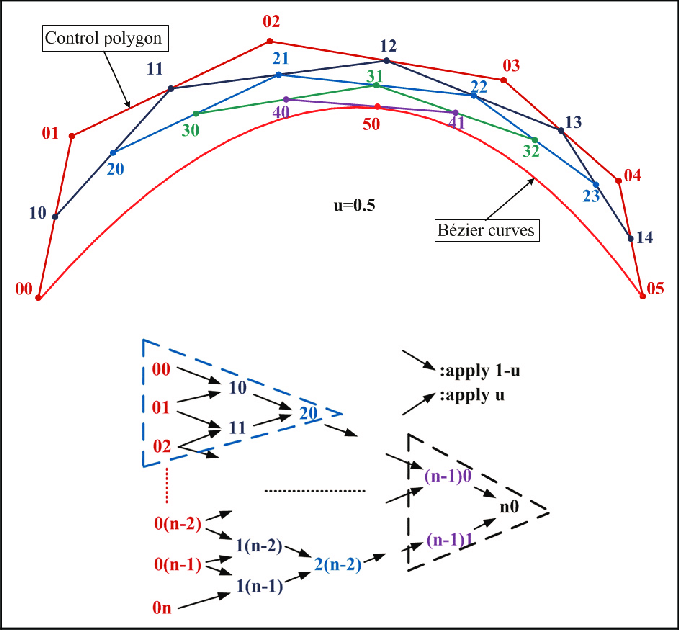
\includegraphics[height=9cm]{figures/General-process-of-De-Casteljau-algorithm.png}
    \caption{De-Casteljau Algorithm, from \cite{Wang-spline}}  
    \label{fig:De-casteljau-algo}
\end{figure}

\subsection{Derivative of Bezier curve}
\label{subsec:Derivative of Bezier curve}
\subsubsection{1st Method}
We use : 
\[
    p^{(k)} = \frac{ n!  }{ \left( n-k\right) ! } \sum_{k=0}^{n-k} \Delta^k P_i B _{ i }^{
    n-k} (t) 
\]
then we calculate $ \Delta ^k P_i  $ given by the De Casteljau algorithm on $ \Delta^kP_i
$.
When k = 0 
\[
\underbrace{
\begin{pmatrix*}
    P_0  \\
    P_1 \\
    \vdots \\
    P_n 
\end{pmatrix*}
\to  
\begin{pmatrix*}
    \Delta P_0  \\
    \Delta P_1 \\
    \vdots \\
    \Delta P_{n-1}  
\end{pmatrix*}
\to 
\begin{pmatrix*}
    \Delta^2 P_0  \\
    \Delta^2 P_1 \\
    \vdots \\ 
    \Delta^2 P_{n-2}  
\end{pmatrix*}}_{ \text{finite differences}} 
\underbrace{
\to 
P''(t) \frac{ 1 }{ n\left( n-1\right)  } }_{\text{De Casteljau}}
\]

\subsubsection{Second Method}
We do not need to calculate $ \Delta^k P_i  $. 
\begin{prop}[]
   \[
       P^{(k)} (t) = \frac{ n!  }{ \left( n-k\right) ! } \Delta ^k P _{ 0 }^{ \left( n-k\right)  } 
   \] 
    \label{def:}
\end{prop}

Thus, for $ k = 1 $ we have 
\[
    P'(t) = n\left( P _{ 1 }^{ (n-1)  } - P _{ 0 }^{ (n-1) } \right) 
\]
k=2 

\[
    P''(t) = n(n-1)\left( P _{ 1 }^{ (n-2)  } -2P _{ 1 }^{ (n-2) } +  P _{ 0 }^{ (n-2) } \right) 
\]
Intuition of the proof : 
\begin{align*}
    \Delta P_0  &= P_1 - P_0  \\
    \Delta P_1  &= P_2 - P_1  \\
    \text{ Which Gives }& \\
     &= \left( 1-t\right) \left( P_1 - P_0 \right) + t\left( P_2 - P_1 \right)  \\ 
      &= \left( 1-t\right) P_1 + tP_2  \\ 
       &= - \left( \left( 1-t\right) P_0 + P_1\right)  \\ 
\end{align*}


\section{Tutorial 2: Bézier Curves and Bernstein polynomials}
\label{sec:Tutorial 2: Bézier Curves and Bernstein polynomials}
\subsubsection{Exercise 1 (Bernstein polynomials)} 
Show the following : 
\begin{enumerate}
    \item Linear precision : 
        \[
            \sum_{i=0}^{n} \frac{ i }{ n  } B^n_i(t) = t \quad \forall t\in [0,1], \
            \forall n > 0, \ \forall i \in \set{ 0,\dots, n } 
        \]
    \item Recursive formula 
        \[
            B^n_i(t) = \left( 1-t\right) B _{ i }^{ n-1 } (t) + tB _{ i-1 }^{ n-1 } (t)
            \quad \forall n > 0, \ \forall i \in \set{ 0, \dots, n } 
        \]
    \item The family of Bézier polynomials $ \left( B_9\right) _{ 0\leq i \leq n  }^{  }
        $ is a basis of the space of polynomials of degree $ \leq n  $. 
\end{enumerate}
\subsubsection{Exercise 2}
Let $ P_0 $ and $ P_1 $ be two points of $ \mathbb{R}^d $. Descrie the Bézier curve
associated to $ P_0 $ and $ P_1 $. 

\subsubsection{Exercise 3}
Let $ \mathcal{ A }  $ be the affine space identified to $ \mathbb{R}^2 $ and $ \gamma $
be the parameterized curve 
\begin{align*}
    \gamma :  [0,1] &\to \mathbb{R}^2  \\ 
     t &\to \left( t,t^2\right)  \\ 
\end{align*}
\begin{enumerate}
    \item Express $ \gamma $ in the monomial basis. 
    \item Express $ \gamma $ in the Bernstein polyonimals basis. 
    \item Give the control polygon of $ \gamma $. Make a drawing with the curve and
        control polygon. 
\end{enumerate}

\subsubsection{Exercise 4}
Let $ [)_0, \cdots, P_6]  $ be a control polygon and : 
\begin{itemize}
  \item Express the condition on the $ P_i $ to ensure that the Bézier curve 
      \[
          P(t) = \sum_{i=0}^{6} P_iB^6_i(t) 
      \]
      is closed of class $ \mathscr{ C } ^2 $.
  \item Draw an example of such a control polygon.
\end{itemize}

\subsubsection{Exercise 5 (Bézier Function) }
A Bézier function is a curve of the form 
\begin{align*}
    f : [0,1] &\to \mathbb{R}\\
    t &\to \sum_{i=0}^{n} \lambda_i B_i^n(t) 
\end{align*}
Show that the graph  $ G(f) \coloneqq \set{ \left( x,f(x)\right) , x \in [0,1] }  $ of the
function $ f $ is a Bézier curve associated to the points $ P_i = \left( i/n, \lambda_i
\right)  $.

\subsubsection{Exercise 6}
Let $ f(t) = \sum_{i=0}^{n} \lambda_iB^n_i(t)  $ be a Bézier function. 
\begin{enumerate}
    \item Show that 
        \[
        \int\limits_{0}^{1} f(t) \ dt = \frac{ \lambda_0 + \dots + \lambda_n }{ n+1 } 
        \]
        hint : consider the primitive F of f
    \item In particular, show that 
        \[
            \int\limits_{0}^{1} B^n_i(t) = \frac{ 1 }{ n+1 } 
        \]
\end{enumerate}
\subsubsection{Exercise 7 (Degree elevation) }
The idea is to use the observation that a polynomial curve $ P $ of degree $ \leq n  $ can
be seen as a polynomial curve of degree $ \leq n+1 $, namely 
\[
    P(t) = \sum_{i=0}^{n} P_iB^n_i(t) = \sum_{i=0}^{n+1} Q_iB _{ i }^{ n+1 } (t) 
\] 
\begin{enumerate}
    \item Show that 
        \[
            B _{ i }^{ n  } (t) = \frac{ n+1 - i }{ n+1 } B _{ i }^{ n+1 } (t) + \frac{
            n+1  }{ i+1 } (t) 
        \]
    \item Calculate $ Q_i $ in terms of the $ P_j $'s
\end{enumerate}


\subsection{Solutions}
\label{subsec:Solutions}
\subsubsection{1) }
\begin{enumerate}
    \item 
        The first index vanishes, so we can rewrite the sum as 
        \[
            \sum_{i=1}^{n} \frac{ i }{ n  }  B _{ i  }^{ n  } (t) 
        \]
        Furthermore, 
        \[
        i \begin{pmatrix*}
            n   \\
            i  
        \end{pmatrix*}
        = \frac{ n\left( n-1\right) !  }{ \left( i-1\right) !\left( n-i\right) ! } = 
        n\begin{pmatrix*}
            n-1  \\
            i-1  
        \end{pmatrix*}
         
        \]
        Thus, we have, for the first iteration of the sum 
        \[
            \frac{ n   }{ n  } \frac{ \left( n-1\right) ! }{ \left( n-1\right) ! }  
            t\left( 1-t\right) ^{n-1} = t\left( 1-t\right) ^{n-1} = t \left( B _{ 0 }^{
            n-1 } (t) \right) 
        \]
        which allows us to rewrite the sum as 
        \[
            t\sum_{i=0}^{n} B _{ i }^{ n  } (t)  = t\left( 1\right) = t
        \]
    \item 
        \begin{align*}
            B _{ i }^{ n  } (t) &= \left( 1-t\right) B _{ i }^{ n-1 } (t) + tB _{ i-1 }^{
            n-1 } (t) \\
                                &= \left( 1-t\right) \begin{pmatrix*}
                                    n-1  \\
                                     i 
                                \end{pmatrix*}
                                t^i\left( 1-t\right)^{n-1-i} + t 
                                \begin{pmatrix*}
                                    n-1  \\
                                    i-1  
                                \end{pmatrix*}
                                t^{i-1}\left( 1-t\right) ^{n-1 - (i-1)}\\ 
                                 &= \begin{pmatrix*}
                                     n-1  \\
                                     i  
                                 \end{pmatrix*}
                                 t^i\left( 1-t\right) ^{n-i} +
                                 \begin{pmatrix*}
                                     n-1  \\
                                     i-1  
                                 \end{pmatrix*}
                                 t^i\left( 1-t\right) ^{n-i}\\
                                  &= \left( \begin{pmatrix*}
                                      n-1  \\
                                      i  
                                  \end{pmatrix*}
                                  + 
                                  \begin{pmatrix*}
                                      n-1  \\
                                      i-1  
                                  \end{pmatrix*}
                              \right) t^i\left( 1-t\right) ^{n-i}  \\
                               &= \begin{pmatrix*}
                                   n   \\
                                   i  
                               \end{pmatrix*}
                               t^i\left( 1-t\right) ^{n-i} = B _{ i }^{ n  } (t) \\ 
            \end{align*}
        \item To show $ B _{ i }^{ n  } (t) $ as a basis of the space of polynomials of
            degree $ \leq n  $ we use derivation. 
            Consider how 
            \[
                B _{ i }^{ n  } (t) \implies \begin{pmatrix*}
                    n   \\
                    i  
                \end{pmatrix*} t^i
                \left( P \right)  
            \]
            where $ P $ is some polynomial. Then we can write this as a sum under the form 
            \[
            \alpha_0\left( P\right) + \alpha_1t\left( P\right) + \cdots  + \alpha_nt^n = 0
            \]
            We check each $ \alpha_i $. Firstly, taking the derivative of this polynomial
            gives us 
            \[
                \alpha_1\left( P\right) + \cdots  + n\alpha_nt^{n-1} = 0
            \]
            Then $ \alpha_0 = 0 $, this can be done iteratively for each $ \alpha_i $.
            Then $ B _{ i  }^{ n  } (t)  $ is a linear independent set and a basis for
            polynomials of degree $ \leq n $.  
\end{enumerate}

\subsubsection{2)}
The Bézier curve consisting of only 2 points is the straight line :  
\begin{align*}
    P(t) &= \sum_{i=0}^{1} P_iB _{ i }^{ n  } (t) \\
     &= P_0\left( 1-t\right) + P_1t \\ 
      &= P_0 + \left( P_1 - P_0\right) t \\ 
\end{align*}

\subsubsection{3)}
\begin{enumerate}
  \item The monomial basis has representation 
      \[
      \begin{pmatrix*}
          1  \\
          0  
      \end{pmatrix*}
      t + \begin{pmatrix*}
          0  \\
          1  
      \end{pmatrix*}
      t^2
      \]
  \item Bernstein basis is given by : 
      \[
          B _{ 0 }^{ 2 } (t) = \left( 1-t\right)^2; \quad B _{ 1 }^{ 2 } (t) = 2t\left( 1-t\right)
           ; \quad B _{ 2 }^{ 2 } (t) = t^2
      \]
      which results in the following : 
     \[
     \begin{pmatrix*}
         0  \\
         0  
     \end{pmatrix*}
     B _{ 0 }^{ 2 } (t) + 
     \begin{pmatrix*}
         \frac{ 1 }{ 2 }   \\
         0 
     \end{pmatrix*}
     B _{ 1 }^{ 2 } (t) + \begin{pmatrix*}
         1  \\
         1  
     \end{pmatrix*}
     B _{ 2 }^{ 2 } (t)
     \]
 \item The curve is given by :  
\begin{figure}[ht]
    \centering
    \incfig{e4p3}
    \caption{e4p3}
    \label{fig:e4p3}
\end{figure}
\end{enumerate}

\subsubsection{4)}
\begin{itemize}
  \item In order to ensure that the Bézier curve 
      \[
          P(t) = \sum_{i=0}^{6} P_iB _{ i }^{ 6 } (t) 
      \]
      to be closed of class $ \mathscr{ C } ^2 $ we must have 
      \begin{enumerate}
          \item $P(0) = P(1)$ 
          \item $ P'(0) = P'(1) $
          \item $ P''(0) = P''(1) $
      \end{enumerate}
      Thus, 
      \begin{enumerate}
          \item \[ P_0 = P_n \]
          \item 
              \begin{align*}
                  P'(0) = 6\left( P_1 - P_0\right) &= P'(1) = 6\left( P_5 - P_6\right) \\
                  \vv{P_1P_0} &= \vv{P_5P_6} 
              \end{align*}
          \item 
              \begin{align*}
                  P''(0) = 30\left( P_2 - 2P_1 + P_0\right) &= P''(1) = 30\left( P_4 - 2P_5
                  + P_6\right) \\
                   &\text{ since } P_0 = P_6 \\ 
                  P_2 - 2P_1 &= P_4 - 2P_5 \\
                  \vv{P_2P_4} &= 2\vv{P_1P_5} \\ 
              \end{align*}
      \end{enumerate}
        This system of equations results in the figure : 
\begin{figure}[ht]
    \centering
    \incfig{t2e4}
    \caption{Closed of Class $ \mathscr{ C } ^2 $}
    \label{fig:t2e4}
\end{figure}
\end{itemize}

\subsubsection{5)}
This is found through simple computation. We take 
\[
P_i = \begin{pmatrix*}
    \frac{ i }{ n  }   \\
    \lambda_i   
\end{pmatrix*}
\]
Then 
\begin{align*}
    \sum_{i=0}^{n } \begin{pmatrix*}
        i/n   \\
        \lambda_i   
    \end{pmatrix*}
    B _{ i  }^{ n  } (t) &= \begin{pmatrix*}
        \sum_{i=0}^{n } \frac{ i }{ n  } B _{ i  }^{ n  } (t)   \\
        \sum_{i=0}^{n } \lambda_i B _{ i  }^{ n  } (t)   
    \end{pmatrix*} \\ 
     &= \begin{pmatrix*}
         t  \\
         f(t)  
     \end{pmatrix*}
      \\ 
\end{align*}

\subsubsection{6)}
\begin{enumerate}
    \item 
    \begin{align*}
        \int\limits_{0}^{1} f(t) \ dt
    \end{align*}
\item 
\end{enumerate}

\subsubsection{7)}
\begin{enumerate}
    \item 
        \begin{align*}
            &\frac{ n+1-i }{ n+1 } B _{ i }^{ n+1 } (t) + \frac{ i+1 }{ n+1 }B _{ i+1 }^{
        n+1 } (t)  \\ 
            &=  \frac{ n+1-i }{ n+1 } \begin{pmatrix*}
                n+1  \\
                i  
            \end{pmatrix*}
            t^i\left( 1-t\right) ^{n+1-i} + \frac{ i+1 }{ n+1 } \begin{pmatrix*}
                n+1  \\
                i+1  
            \end{pmatrix*}
            t^{i+1}\left( 1-t\right) ^{n+1-(i+1)} \\ 
            &=  
                \frac{ n! }{ i!\left( n-i\right) ! } 
            t^i\left( 1-t\right) ^{n+1-i} + 
            \frac{n! }{ i!\left( n - i\right)!} 
            t^{i+1}\left( 1-t\right) ^{n-i} \\ 
             &= \begin{pmatrix*}
                 n   \\
                 i  
             \end{pmatrix*}
             t^i\left( 1-t\right) ^{n-i} \left( \left( 1-t\right) + t\right)    
             \\
             &= B _{ i  }^{ n  } (t) \\  
               \\ 
        \end{align*} 
    \item We begin by expanding using the form above : 
        \begin{align*}
            \sum_{i=0}^{n } P_iB _{ i }^{ n  } (t) &= \sum_{i=0}^{n }P_i \left( \frac{ n+1-i
            }{ n+1 }B _{ i }^{ n+1 } (t) + \frac{ i+1 }{ n+1 } B _{ i+1 }^{ n+1 }
        (t)\right) \\
                                                   &= \sum_{i=0}^{n} \frac{ n+1-i }{ n+1 }
                                                   P_iB _{ i }^{ n+1 } (t) +
                                                   \sum_{i=1}^{n+1} \frac{ i }{ n+1 } 
                                                   P_{i-1}B _{ i }^{ n+1 }  \\ 
                                                   &= P_0B _{ 0 }^{ n+1 } (t) +
                                                   \sum_{i=1}^{n} \left( P_i \frac{ n+1-i
                                                   }{ n+1 } + P_{i-1} \frac{ i }{ n+1 }
                                               \right) B _{ i }^{ n+1 } (t) + P_nB _{ n+1
                                           }^{ n+1 }  \\ 
        \end{align*} 
\end{enumerate}


